% =====================================================================
% ICAI 2026 -- Anonymous Submission
% 9th International Conference on Applied Informatics
% Springer LNCS/CCIS template
% =====================================================================
\documentclass[runningheads]{llncs}

\usepackage[T1]{fontenc}
\usepackage[utf8]{inputenc}
\usepackage{graphicx}
\usepackage{booktabs}
\usepackage{array}
\usepackage{amsmath,amssymb}
\usepackage[protrusion=true,expansion=false]{microtype}
\usepackage[hidelinks]{hyperref}
\usepackage{xcolor}
\usepackage{caption}
\usepackage{subcaption}
\usepackage{url}

\graphicspath{{figs/}}

% Sensible widths for tables
\newcolumntype{L}[1]{>{\raggedright\arraybackslash}p{#1}}

% =====================================================================
\begin{document}

\title{Securing Federated TinyML Intrusion Detection for IoT/MQTT Networks with ASCON-128 in an Edge--Fog--Cloud Architecture}

% --- Anonymous block (first submission) ---
\titlerunning{Federated TinyML IDS with ASCON-128 for IoT/MQTT}
\author{Anonymous Authors}
\authorrunning{Anonymous}
\institute{Anonymous Institution\\
\email{anonymous@example.com}}

\maketitle

% =====================================================================
\begin{abstract}
Intrusion detection in resource-constrained IoT/MQTT networks must
simultaneously address three goals that the literature usually studies in
isolation: low-footprint inference on microcontrollers, privacy-preserving
distributed training, and authenticated communication of model artifacts.
We present an end-to-end Edge--Fog--Cloud system that integrates the three
on real hardware. An ESP32-S3 executes a compact 1{,}139-parameter TinyML
classifier ($\approx$4.5\,kB) over thirteen flow features, while a Raspberry
Pi~4 gateway performs local training and a PC server coordinates
hierarchical federated learning (HFL) with weighted FedAvg.
All control and weight-exchange channels are protected with NIST-standardized
ASCON-128 authenticated encryption. Eight experimental variants are evaluated
by crossing three binary axes (model architecture: MLP vs.\ CNN-1D; security:
ASCON vs.\ plain JSON; topology: with vs.\ without a Fog leader/peer layer),
yielding 58 federated runs consolidated under a unified site-reliability
engineering (SRE) telemetry layer. The best configuration
(\texttt{CNN\_ASCON\_FOG}) reaches 0.975 global accuracy with an
ASCON-induced temporal overhead between 0.10\,\% and 0.27\,\% of the
federated round and a $\approx$48\,\% per-message size overhead. Variants
with authenticated encryption do not degrade convergence over the evaluated
testbed, and the Fog topology improves accuracy when combined with ASCON
but can hurt it without authentication. We discuss the validity boundaries of
these findings, including the closed three-class label set, the heuristic
gateway labeller, and the limited testbed scale.

\keywords{IoT Security \and MQTT \and TinyML \and
Hierarchical Federated Learning \and ASCON-128 \and Lightweight Cryptography
\and Edge--Fog--Cloud \and Intrusion Detection System.}
\end{abstract}

% =====================================================================
\section{Introduction}
\label{sec:intro}

The expansion of Internet of Things (IoT) and Industrial IoT (IIoT)
deployments has enlarged the network attack surface of homes, laboratories,
and industrial sites that increasingly rely on lightweight publish/subscribe
protocols such as MQTT~\cite{ni2024iiot,amanullah2020deep}. Detecting
intrusions in those environments is challenging on at least three
independent dimensions: (i)~edge devices have severe memory and energy
constraints; (ii)~centralising traffic captures into a single server is
incompatible with the privacy and bandwidth profile of many deployments;
and (iii)~the federated training loop itself --- model updates, control
messages, deployment events --- becomes a sensitive asset that must be
protected in transit.

Existing solutions tend to address these dimensions \emph{separately}: a
substantial body of work studies TinyML-based intrusion detection on
microcontrollers~\cite{dini2024embedded,heydari2025tinyml}, a parallel line
studies federated learning (FL) for IoT
security~\cite{imteaj2022survey,ficco2024fl}, and a third one analyses
lightweight authenticated encryption such as
ASCON~\cite{nist2025ascon,kaur2025ascon}. Few works measure all three
together on physical hardware. The recently
selected NIST ASCON standard~\cite{nist2025ascon} provides a 128-bit
authenticated encryption-with-associated-data (AEAD) primitive specifically
designed for constrained devices, but its empirical cost inside a real
federated cycle on IoT MCUs is rarely reported end-to-end.

This paper addresses that integration gap and makes three contributions:

\begin{enumerate}
  \item \textbf{An Edge--Fog--Cloud IDS architecture} for IoT/MQTT
        networks, built on ESP32-S3 nodes, Raspberry Pi~4 gateways and a
        PC coordinator, with two interchangeable topologies (a standard
        Edge$\rightarrow$Fog$\rightarrow$Cloud chain and a Fog
        \emph{leader/peer} pre-aggregation variant).
  \item \textbf{A lightweight federated TinyML pipeline} where only the
        last two dense layers of the on-device classifier (163~parameters,
        652~bytes) are exchanged through weighted FedAvg, exported as
        embeddable C++ arrays for on-board inference without dynamic
        memory allocation.
  \item \textbf{An ASCON-128 protected federated cycle} with measured
        latency and payload overhead against a functionally equivalent
        PLAIN baseline, evaluated jointly on the eight combinations of
        model, security and topology over 58 federated runs.
\end{enumerate}

We do \emph{not} claim that ASCON improves classification accuracy or that
the system solves IoT security in general. The empirical contribution is
the measurement of viability and overhead of the joint stack under a
clearly stated threat model.

The rest of the paper is organised as follows. Section~\ref{sec:related}
positions the work in the literature. Section~\ref{sec:arch} describes the
Edge--Fog--Cloud architecture. Section~\ref{sec:fl} details the federated
TinyML pipeline. Section~\ref{sec:ascon} covers the ASCON-128 security
layer. Section~\ref{sec:setup} presents the experimental setup, and
Section~\ref{sec:results} reports the results. Section~\ref{sec:threats}
discusses threats to validity, and Section~\ref{sec:conclusion} concludes
and outlines future work.

% =====================================================================
\section{Related Work}
\label{sec:related}

\paragraph{TinyML for IDS on MCUs.}
Dini~\textit{et~al.}~\cite{dini2024embedded} survey AI-model toolchains
(TensorFlow Lite Micro, STM32Cube.AI, Vitis~AI) and show that successful
integration on a microcontroller depends as much on the
hardware/software stack as on the model itself. Tekin
\textit{et~al.}~\cite{tekin2023energy} insist that on-device IDS work must
report memory, latency and energy together with classification accuracy;
Heydari and Mahmoud~\cite{heydari2025tinyml} confirm this on smart-home
hardware. Most reported pipelines still rely on capable servers and do not
demonstrate deployment on real MCUs.

\paragraph{Federated learning for IoT security.}
Federated approaches reduce the need to centralise raw traffic, but
introduce non-IID data, partial participation and communication overhead
\cite{imteaj2022survey,albanbay2025,roy2023adapted}. Hajj
\textit{et~al.}~\cite{hajj2023crosslayer} demonstrate a cross-layer
federated IDS for IoT, while Ficco \textit{et~al.}~\cite{ficco2024fl}
validate FL with transfer learning for on-board training on ESP32 and
Raspberry Pi class devices. Tran \textit{et~al.}~\cite{tran2026edgetrust}
quantify a memory gap of up to three orders of magnitude between
Byzantine-robust aggregators (Krum, FLTrust, Fed-NGA) and typical MCU SRAM,
arguing for hierarchical decomposition. Our work adopts that hierarchical
view but focuses on confidentiality and integrity rather than Byzantine
robustness.

\paragraph{Lightweight cryptography in the federated cycle.}
The NIST 800-232 standard formalises the ASCON
family~\cite{nist2025ascon}; Kaur \textit{et~al.}~\cite{kaur2025ascon}
provide a comprehensive survey of ASCON implementations, attacks and
countermeasures. In contrast, Mirzaali \textit{et~al.}~\cite{mirzaali2025lwc}
show experimentally on three Raspberry Pi devices that ad-hoc
ultra-lightweight permutations used for authentication can be broken by
disclosure and desynchronisation attacks, even when the protocol structure
looks sound. These two references jointly motivate adopting a standardised
AEAD inside the federated cycle and treating side-channel hardening as
future work.

\paragraph{Gap.}
Existing work covers each of these three axes separately. We are not aware
of a study that measures, on the same physical IoT testbed, the joint
behaviour of TinyML inference, hierarchical federated training and
authenticated lightweight encryption, with explicit comparison against a
functionally equivalent plaintext baseline. This paper fills that gap.

% =====================================================================
\section{System Architecture}
\label{sec:arch}

\begin{figure}[t]
  \centering
  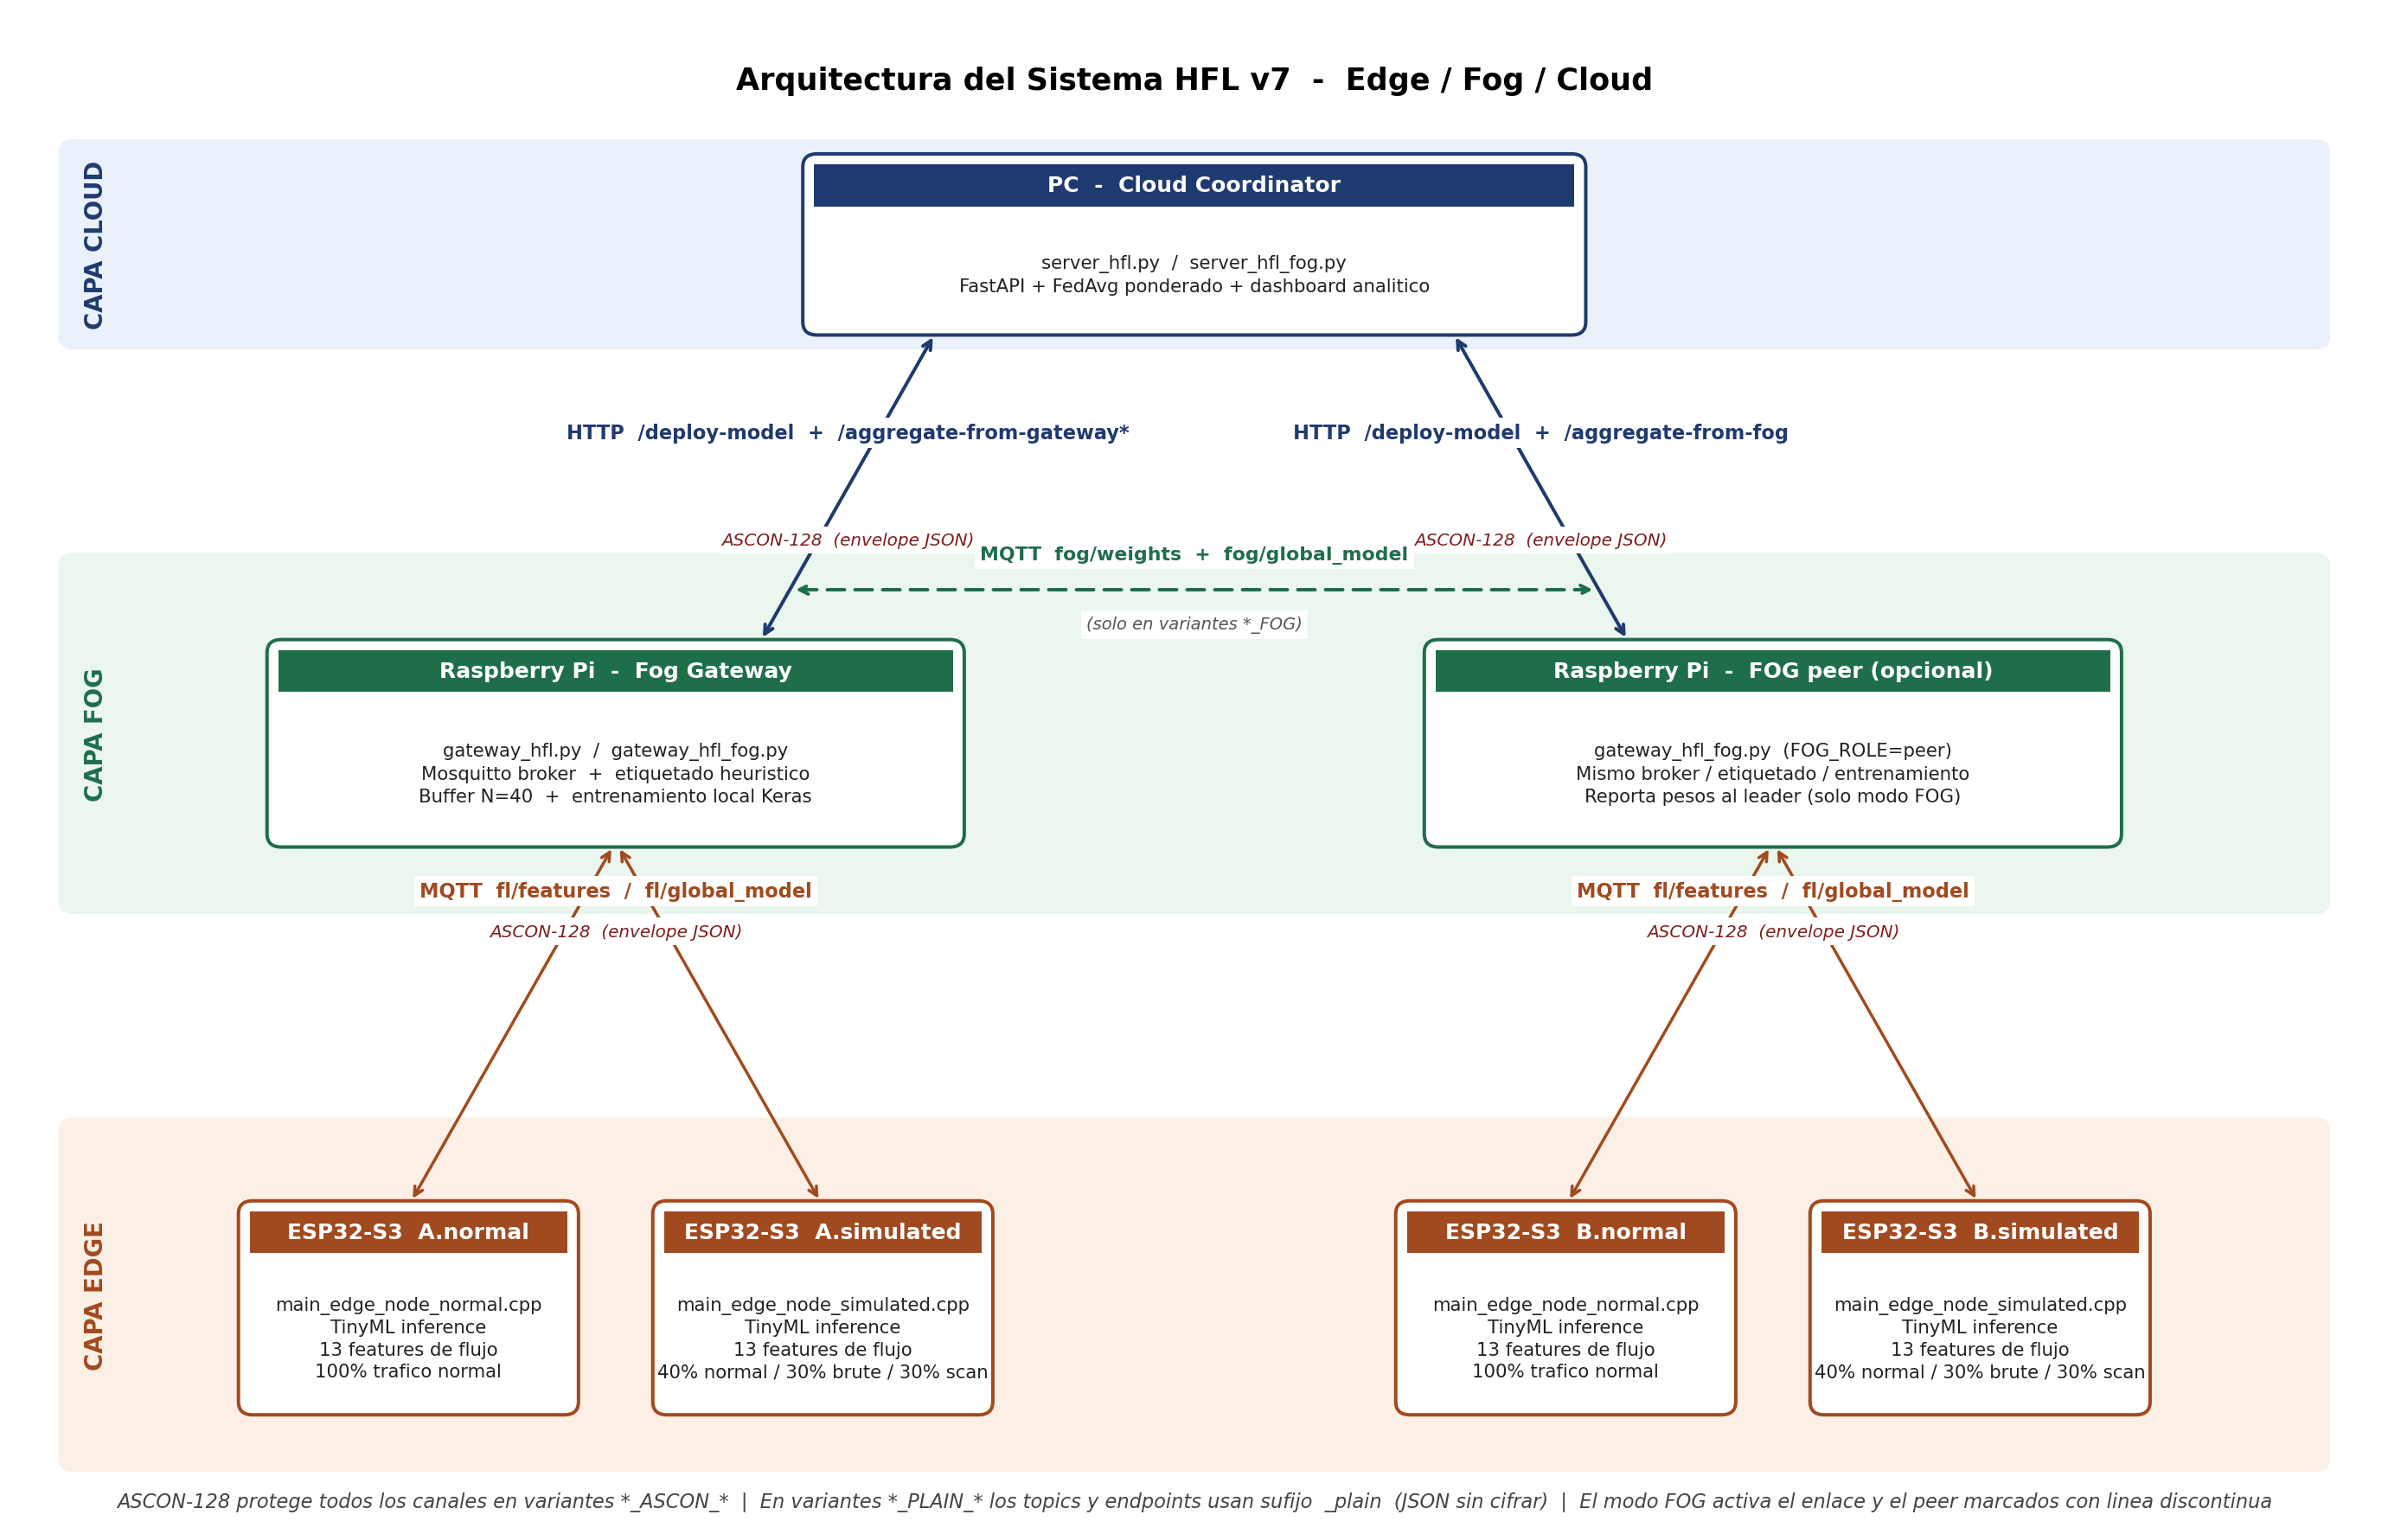
\includegraphics[width=0.95\linewidth]{fig_architecture.png}
  \caption{Edge--Fog--Cloud architecture of the proposed IDS. The dashed
  links are active only in the Fog (leader/peer) topology variant; all
  channels are protected with ASCON-128 in the \texttt{*\_ASCON\_*}
  variants.}
  \label{fig:arch}
\end{figure}

The system is organised in three hierarchical layers (Fig.~\ref{fig:arch})
that map onto the Edge, Fog and Cloud roles common in IoT references
\cite{wang2019datafusion,tran2026edgetrust}. Each layer has a single
responsibility, and the entire control and data plane is defined in terms
of MQTT and HTTP exchanges, so the layers can be replaced independently.

\paragraph{Edge layer.}
Two ESP32-S3 microcontrollers per gateway publish features to the local
Mosquitto broker via the \texttt{fl/features} topic. Each node executes a
1{,}139-parameter MLP classifier ($\approx$4.5\,kB) on thirteen flow
features (packet counts, mean packet length, inter-arrival statistics, TCP
flags) and reports per-flow predictions and feature vectors at a fixed
cadence. To exercise heterogeneity, one node emits exclusively
\emph{normal} traffic, while a second node emits a calibrated mixture
(40\,\% \emph{normal}, 30\,\% \emph{mqtt\_bruteforce}, 30\,\% \emph{scan\_A}).
No on-device training is performed on the MCU: the ESP32-S3 runs only
inference and ASCON-128 in native C++.

\paragraph{Fog layer.}
A Raspberry Pi~4 acts simultaneously as the Mosquitto broker, the local
trainer and an HTTP bridge to the coordinator. Incoming feature vectors
are labelled by a heuristic rule (Section~\ref{sec:fl}), accumulated into a
buffer of $N_s = 30$ samples, used to train the federated layers of the
classifier for $E = 5$ local epochs, and finally serialised together with
the local accuracy and sample count for transmission to the PC server. In
the Fog topology variant a second Raspberry Pi participates as a
\emph{peer}: it ships its local weights to the \emph{leader} through the
\texttt{fog/weights} topic, the leader applies an intermediate FedAvg and
sends the pre-aggregated update to the cloud, then redistributes the
received global model through \texttt{fog/global\_model}.

\paragraph{Cloud layer.}
A FastAPI server (\texttt{server\_hfl.py} or \texttt{server\_hfl\_fog.py})
collects updates from $K = 2$ gateways, performs a weighted FedAvg, and
publishes the new global model back to the gateways through HTTP
(\texttt{/deploy-model}). It also acts as the sink for the SRE telemetry
described later. The server is assumed to be inside the trusted computing
base and is the only point that observes weights from \emph{all} gateways.

\paragraph{Threat model.}
We assume a passive or active network attacker that can eavesdrop or modify
wireless traffic between the ESP32 nodes, the Raspberry Pi gateways and the
PC coordinator, but cannot compromise the endpoints. ASCON-128 over every
channel addresses confidentiality and integrity of features, weights and
control messages; nonces are constructed from a 32-bit truncated timestamp
and a monotonic counter to detect replay. Out of scope for this paper are
Byzantine clients and data poisoning, physical side-channel attacks against
ASCON, and membership inference over the federated weights; these
limitations are discussed explicitly in Section~\ref{sec:threats}.

% =====================================================================
\section{Federated TinyML Pipeline}
\label{sec:fl}

\subsection{On-device classifier}

The on-device classifier is a fully connected network with
$13 \rightarrow 32 \rightarrow 16 \rightarrow 8 \rightarrow 3$ topology
(Table~\ref{tab:mlp}), totalling 1{,}139 parameters in 32-bit floating
point ($\approx$4.5\,kB), which fits comfortably in the ESP32-S3 SRAM
without quantisation. The federated cycle exchanges only the last two
dense layers (\texttt{W3}, \texttt{b3}, \texttt{W4}, \texttt{b4}, a total
of 163 parameters or 652~bytes per round); the lower layers are trained
offline and frozen on the device. A second branch replaces the dense lower
block with a 1D-CNN (\texttt{Conv1D(32)} $\rightarrow$ \texttt{Conv1D(16)}
$\rightarrow$ GAP) whose convolutional and BatchNorm layers are fused and
kept fixed on the MCU, leaving the same federated dense block as the only
trainable head. Federating only the final layers follows the FL+TL
strategy reported in \cite{ficco2024fl,roy2023adapted} and bounds the
payload size irrespective of the underlying architecture.

\begin{table}[t]
\centering
\caption{Parameter distribution of the on-device MLP classifier. Federated
layers (in italics) are the only ones exchanged each round.}
\label{tab:mlp}
\small
\begin{tabular}{@{}lrrr@{}}
\toprule
Layer & Input & Output & Parameters \\
\midrule
Dense 1 (ReLU)              & 13 & 32 & $13 \times 32 + 32 = 448$ \\
Dense 2 (ReLU)              & 32 & 16 & $32 \times 16 + 16 = 528$ \\
\emph{Dense 3 (ReLU, fed.)} & 16 &  8 & $16 \times 8  + 8  = 136$ \\
\emph{Dense 4 (Softmax, fed.)} & 8 & 3 & $8  \times 3  + 3  = 27$  \\
\midrule
\textbf{Total} & & & \textbf{1{,}139} \\
\bottomrule
\end{tabular}
\end{table}

\subsection{Hierarchical FedAvg protocol}

Each gateway accumulates $N_s = 30$ labelled samples per round and trains
locally for $E = 5$ epochs. The PC server then applies weighted FedAvg:
\begin{equation}
\mathbf{W}_{\text{global}}^{(t+1)} =
\sum_{k=1}^{K} \frac{n_k}{\sum_{j=1}^{K} n_j}\,\mathbf{W}_k^{(t)},
\label{eq:fedavg}
\end{equation}
where $n_k$ is the number of samples used in gateway $k$'s local update
and $\mathbf{W}_k^{(t)}$ are its federated weights at round $t$. In the
Fog variant Eq.~\ref{eq:fedavg} is first applied locally at the leader on
the messages received from its peers, and the resulting pre-aggregated
update is sent to the PC server.

Labels are assigned at the gateway by a heuristic calibrated on the
distribution of the public datasets:
\texttt{num\_pkts} $\geq$ 50 and \texttt{num\_psh} $\geq$ 10 produces the
\emph{bruteforce} label; \texttt{num\_pkts} $\leq$ 5 with small
\texttt{mean\_pkt\_len} and at least one PSH produces \emph{scan\_A};
otherwise the sample is mapped to \emph{normal} if the byte counts fall in
the expected range, and discarded otherwise. This heuristic is a known
source of label noise and is treated explicitly as a validity threat
(Section~\ref{sec:threats}).

\subsection{Datasets and classes}

The system targets three traffic classes (\emph{normal},
\emph{mqtt\_bruteforce}, \emph{scan\_A}) selected because they are
representative of what a single MQTT-enabled node may observe in a smart
home or laboratory setting. The classes are derived from public IoT/IDS
corpora such as MQTT-IoT-IDS2020 and TON\_IoT
\cite{moustafa2020toniot,ferrag2022edgeiiotset,neto2023ciciot} after
unifying schemas and converting captures into the 13-dimensional flow
feature space described above. A central training set with 256{,}276 flows
is reserved for the centralised classical baselines reported in
Section~\ref{sec:results}.

% =====================================================================
\section{ASCON-128 Security Layer}
\label{sec:ascon}

ASCON-128 provides authenticated encryption with associated data (AEAD)
using a 128-bit pre-shared symmetric key, a 128-bit nonce constructed
from a truncated timestamp and a monotonic counter, and a 128-bit
authentication tag. We chose the original ASCON-128 specification
(64-bit rate) over ASCON-128a (128-bit rate) because the payload sizes in
the system (13 floats for features and $\sim$3.6\,kB for weight messages)
are small enough that the throughput difference is dominated by other
factors, while the higher number of permutation rounds in ASCON-128
preserves the security margin recently revisited by Kaur
\textit{et~al.}~\cite{kaur2025ascon}.

We protect the four (or, in the Fog variant, six) channels of the system,
shown in Table~\ref{tab:channels}. Both implementations --- the native C++
header used on the ESP32-S3 and the Python implementation used on
Raspberry Pi and PC --- share test vectors so interoperability is
guaranteed across architectures. The encrypted payload is encapsulated in
a JSON envelope with three base64-encoded fields:
\verb|{"ct": "...", "tag": "...", "nonce": "..."}|, exactly as in
\cite{nist2025ascon}. All encryption and decryption operations are
instrumented with high-resolution timers (\texttt{micros()} on the MCU,
\texttt{time.perf\_counter()} in Python) and persisted in a CSV log together
with the federated round identifier and payload sizes, enabling the
overhead breakdown reported in Section~\ref{sec:results}.

\begin{table}[t]
\centering
\caption{Communication channels protected by ASCON-128.}
\label{tab:channels}
\small
\begin{tabular}{@{}llL{4cm}l@{}}
\toprule
Channel & Protocol & Content & Implementation \\
\midrule
ESP32 $\rightarrow$ RPi   & MQTT & Feature vectors (13 floats) & C++ \\
RPi $\rightarrow$ PC      & HTTP & Local weights + metrics    & Python \\
PC $\rightarrow$ RPi      & HTTP & Global model               & Python \\
RPi $\rightarrow$ ESP32   & MQTT & Global model               & Python $\rightarrow$ C++ \\
\midrule
\multicolumn{4}{@{}l}{\emph{Fog topology additionally enables:}} \\
peer $\rightarrow$ leader & MQTT & Local weights (pre-agg.)   & Python \\
leader $\rightarrow$ peer & MQTT & Global model (re-dist.)    & Python \\
\bottomrule
\end{tabular}
\end{table}

A PLAIN baseline branch (\texttt{hfl\_v7-no-ascon}) is kept synchronised
with the secure branch and ships the same JSON payloads without
encryption, so that overhead in time and bytes can be attributed solely to
the cryptographic layer.

% =====================================================================
\section{Experimental Setup}
\label{sec:setup}

The testbed consists of four ESP32-S3 microcontrollers (two per gateway),
two Raspberry Pi~4 (4\,GB) acting as gateways and, in the Fog variant, as
leader/peer, and a single PC running the coordinator and SRE telemetry
sink. All devices share a private 2.4\,GHz Wi-Fi network. The same
hardware is reused across all variants so observed differences can be
attributed to a single design axis at a time.

We instantiate the full $2^3 = 8$ factorial design across three binary
axes: model architecture (RN $\equiv$ MLP vs.\ CNN-1D), security mode
(ASCON-128 vs.\ PLAIN), and topology (NoFOG vs.\ FOG), summarised in
Table~\ref{tab:variants}. Each variant is run at least 20~federated rounds
and replicated up to 8~times. The unified telemetry layer
(\texttt{Analisis de Modelos/Completo/}) records per-round accuracy and
loss, per-channel transport latency at the p95 percentile, per-message
plaintext and ciphertext sizes, and a canonical event stream, producing 58
runs in total after consolidation.

\begin{table}[t]
\centering
\caption{Experimental variants. Cells indicate the value of each design
axis; \emph{Purpose} states the comparison each variant enables.}
\label{tab:variants}
\small
\begin{tabular}{@{}llllL{4.3cm}@{}}
\toprule
ID & Edge model & Security & Topology & Purpose \\
\midrule
E1 & MLP (RN)  & ASCON-128 & NoFOG & Reference integral system \\
E2 & MLP (RN)  & PLAIN     & NoFOG & Isolate ASCON cost in RN \\
E3 & MLP (RN)  & ASCON-128 & FOG   & Fog with authenticated RN \\
E4 & MLP (RN)  & PLAIN     & FOG   & Fog without authentication, RN \\
E5 & CNN-1D    & ASCON-128 & NoFOG & Effect of model change \\
E6 & CNN-1D    & PLAIN     & NoFOG & Isolate ASCON cost in CNN \\
E7 & CNN-1D    & ASCON-128 & FOG   & Best-case configuration \\
E8 & CNN-1D    & PLAIN     & FOG   & Fog without authentication, CNN \\
\bottomrule
\end{tabular}
\end{table}

Performance is evaluated along four orthogonal axes: classification
quality (accuracy, F1 macro and weighted, precision, recall, MCC),
cryptographic overhead (encryption/decryption time, byte and percentage
increase per message, fraction of the federated round), federated
efficiency (rounds to convergence, accuracy per round, communication cost
per round), and edge viability (model footprint and inference latency on
the ESP32-S3).

% =====================================================================
\section{Results and Discussion}
\label{sec:results}

\subsection{Centralised baselines and lightweight model comparison}

Classical centralised models trained on the full 256{,}276-flow corpus
(80/20 stratified split, 5-fold cross-validated hyperparameter search)
establish the achievable ceiling. Random Forest reaches an accuracy of
0.9994 with an F1-weighted of 0.9994 and an MCC of 0.9989, followed by
Decision Tree (0.9987) and SVM-RBF (0.9968); linear models drop by 5--6
points, confirming that the decision boundaries between the three classes
are not linearly separable in the 13-feature space. Random Forest and
SVM-RBF, however, exceed the 512\,kB SRAM of the ESP32-S3 by orders of
magnitude and are not deployable as on-device classifiers.

An offline comparison of MCU-compatible architectures over the same
features (MLP, CNN-1D, Residual-MLP, Tiny Transformer) places the three
viable architectures within $\pm$0.6 percentage points of 0.905 accuracy.
The MLP is retained as the primary on-device classifier for its smaller
inference cost, while the CNN-1D is preserved as a second iteration to
study whether higher expressive capacity translates into a real advantage
inside the federated loop.

\subsection{Federated convergence}

\begin{figure}[t]
  \centering
  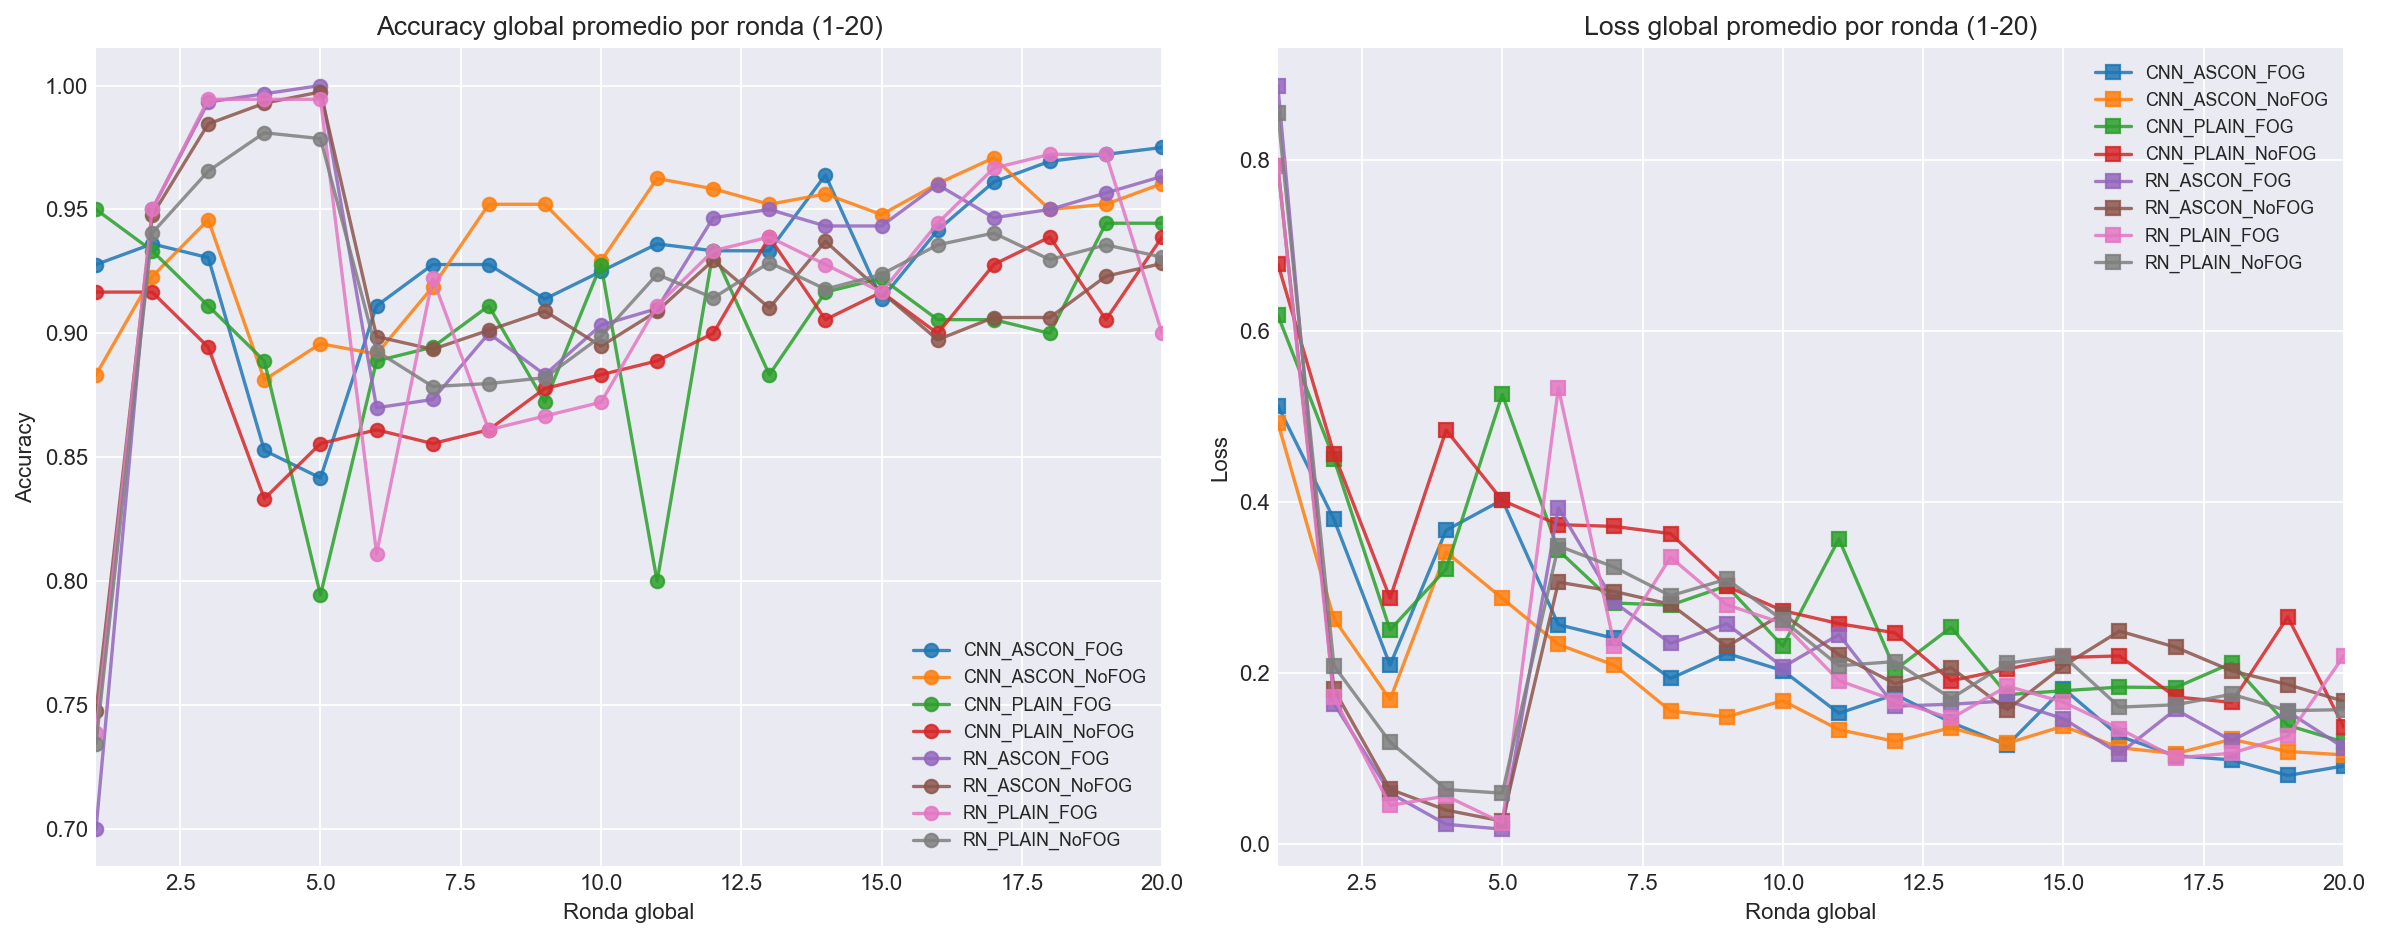
\includegraphics[width=\linewidth]{fig_accuracy_loss.png}
  \caption{Global accuracy (left) and global loss (right) averaged across
  attempts for each variant, rounds 1--20. All variants cross 0.90
  accuracy between rounds 5 and 10; CNN variants stabilise at a higher
  plateau.}
  \label{fig:acc_loss}
\end{figure}

Fig.~\ref{fig:acc_loss} shows the per-round trajectory of accuracy and
loss for the eight variants over the first twenty rounds. Convergence is
reached between rounds 5 and 10 across all variants; the loss drops from
$\approx$0.8 to the 0.1--0.2 range in the same window. The CNN variants,
in particular \texttt{CNN\_ASCON\_FOG} and \texttt{CNN\_ASCON\_NoFOG},
exhibit a more expressive weight trajectory (Fig.~\ref{fig:weights}):
\texttt{w3\_mag} and the class-associated rows \texttt{w4\_brute} and
\texttt{w4\_scan} grow steadily, while the RN variants stabilise early
around \texttt{w3\_mag}~$\approx$~0.29. No variant diverges in the first
twenty rounds; the noisiest behaviour appears in \texttt{w4\_normal} of
\texttt{CNN\_PLAIN\_NoFOG}, which is consistent with the absence of both
Fog aggregation and authenticated tag verification.

\begin{figure}[t]
  \centering
  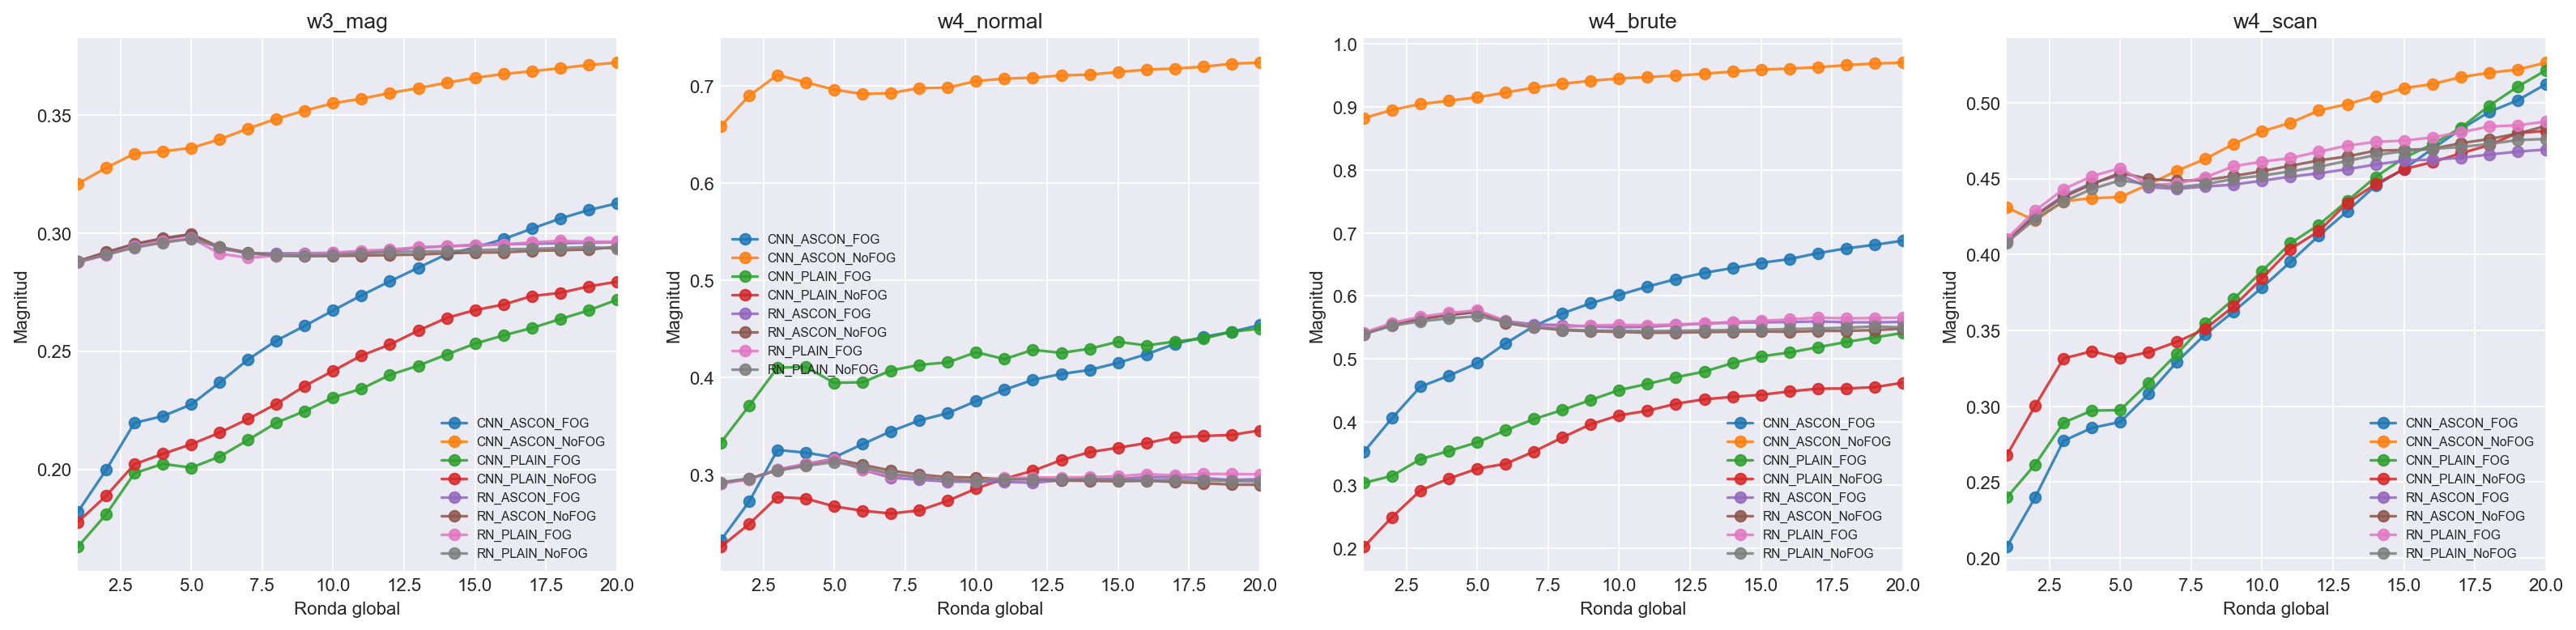
\includegraphics[width=\linewidth]{fig_weight_trends.png}
  \caption{Mean magnitude of the four federated weight tensors per variant
  across rounds 1--20.}
  \label{fig:weights}
\end{figure}

\subsection{Comparison across variants}

Table~\ref{tab:variants_results} summarises the eight variants. The best
configuration is \texttt{CNN\_ASCON\_FOG} with a final accuracy of 0.9750
and final loss of 0.0910, beating its PLAIN counterpart by 3.0 points and
its NoFOG counterpart by 1.5 points. The most striking pairwise comparison
appears in the RN family: \texttt{RN\_ASCON\_FOG} reaches 0.9633 against
0.9000 for \texttt{RN\_PLAIN\_FOG}, a 6.3-point gap. This is consistent
with the hypothesis that authenticated-tag verification filters out
corrupted or duplicate messages before they enter the local training
buffer; however, our experiments do not include controlled fault
injection, so we report this only as an observation and not a causal
claim.

\begin{table}[t]
\centering
\caption{Summary of the eight HFL variants. \textit{GW p95}: p95
decryption latency at the gateway (ESP32~$\rightarrow$~RPi).
\textit{Srv p95}: p95 decryption latency at the server
(RPi~$\rightarrow$~PC). \textit{Overhead}: mean bytes added by the
ASCON+Base64 envelope (zero for PLAIN by construction).}
\label{tab:variants_results}
\small
\begin{tabular}{@{}lrrrrrr@{}}
\toprule
Variant & Acc.\ & Loss & Round (s) & GW p95 & Srv p95 & Ovh.\ (B) \\
\midrule
CNN ASCON FOG    & 0.9750 & 0.091 & 58.6 & 4.53 & 37.5 & 1098 \\
CNN ASCON NoFOG  & 0.9604 & 0.104 & 59.0 & 4.55 & 24.5 & 1049 \\
CNN PLAIN FOG    & 0.9444 & 0.119 & 54.9 & 0.16 & 50.5 & ---  \\
CNN PLAIN NoFOG  & 0.9389 & 0.136 & 52.0 & 0.15 &  0.0 & ---  \\
RN ASCON FOG     & 0.9633 & 0.112 & 71.1 & 4.37 & 50.5 & 1084 \\
RN ASCON NoFOG   & 0.9381 & 0.154 & 72.9 & 4.65 & 26.7 & 1050 \\
RN PLAIN FOG     & 0.9000 & 0.220 & 67.1 & 0.16 &  0.0 & ---  \\
RN PLAIN NoFOG   & 0.9298 & 0.158 & 51.0 & 0.17 &  0.0 & ---  \\
\midrule
\textbf{Mean (8)} & 0.9437 & 0.138 & 61.3 & 2.34 & 17.4 & 636 \\
\bottomrule
\end{tabular}
\end{table}

Disaggregated by class, the best variant exhibits a macro-F1 of
$\approx$0.972 and weighted-F1 of $\approx$0.975, with per-class recall
above 0.96 in all three classes (slightly lower for \emph{scan\_A} where
short burst flows partially overlap statistically with low-intensity
\emph{normal} traffic). The MCC value is $\approx$0.96, confirming that
the global accuracy is not inflated by the majority class.

\subsection{Cryptographic overhead}

\begin{figure}[t]
  \centering
  \begin{subfigure}{0.49\linewidth}
    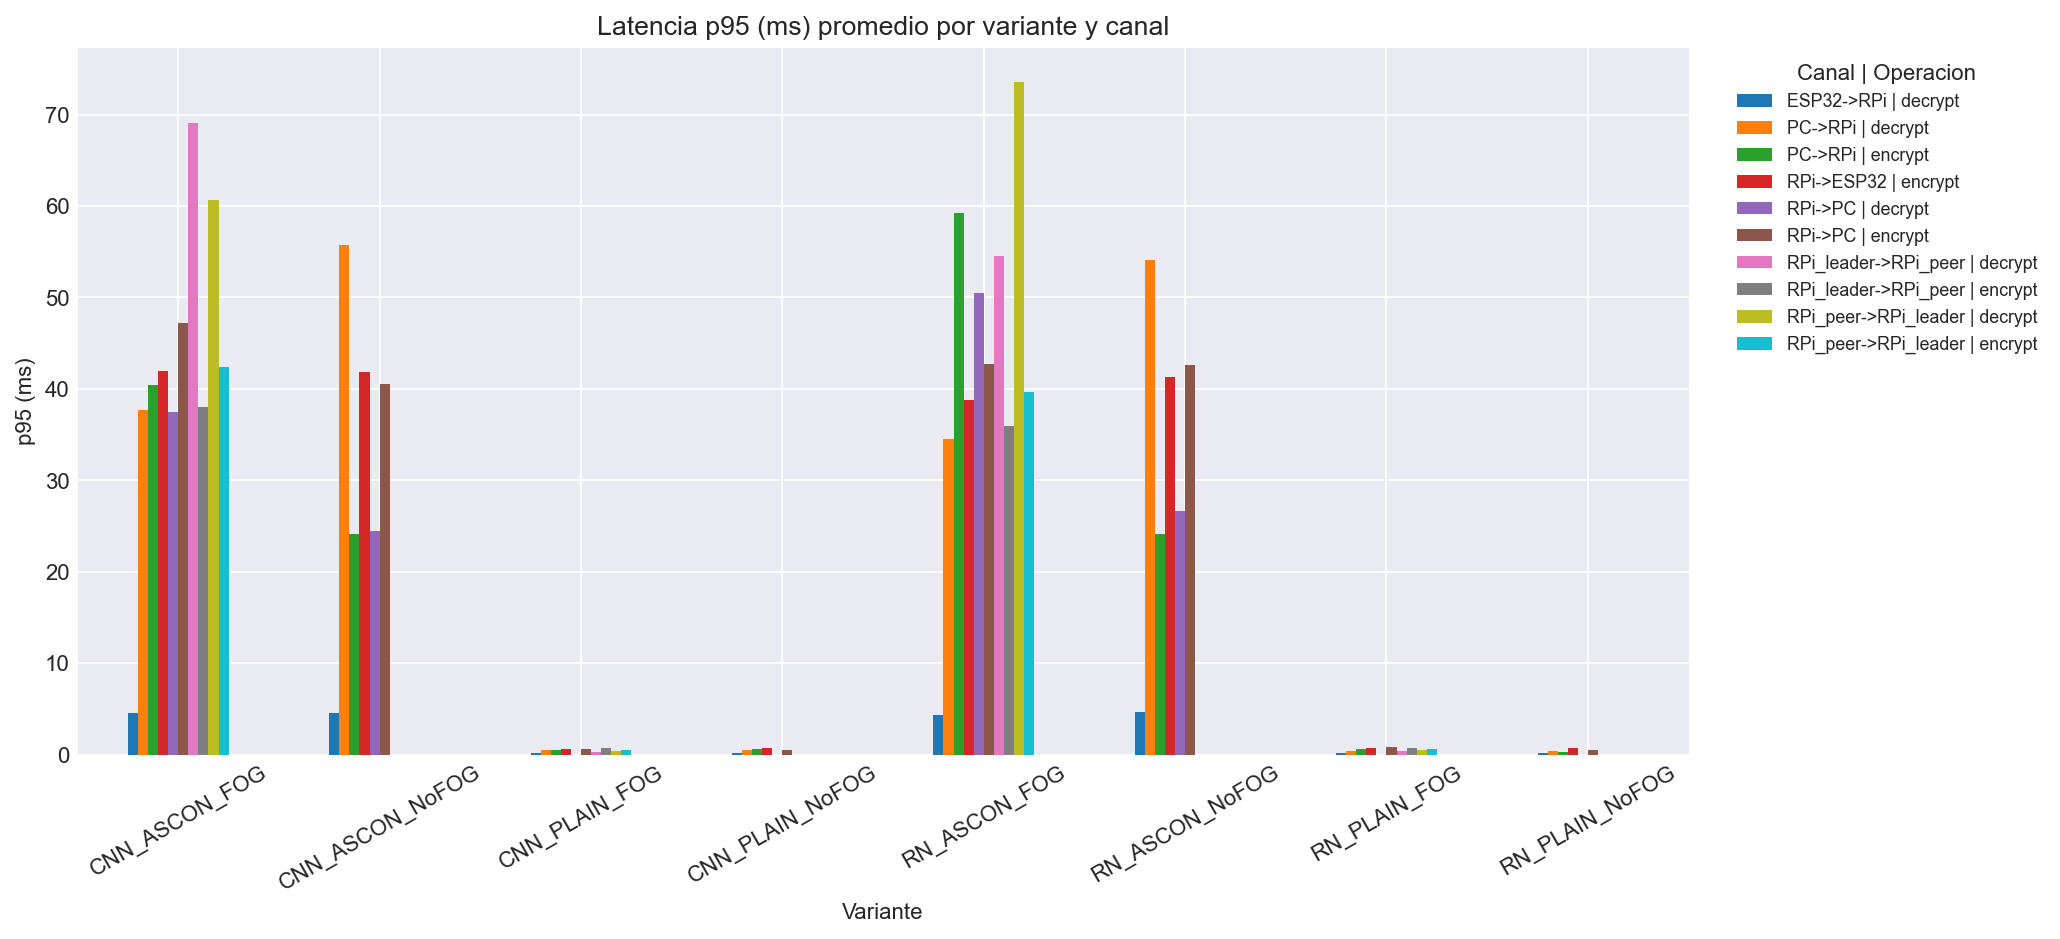
\includegraphics[width=\linewidth]{fig_latency.png}
    \caption{p95 latency per channel/operation.}
  \end{subfigure}
  \begin{subfigure}{0.49\linewidth}
    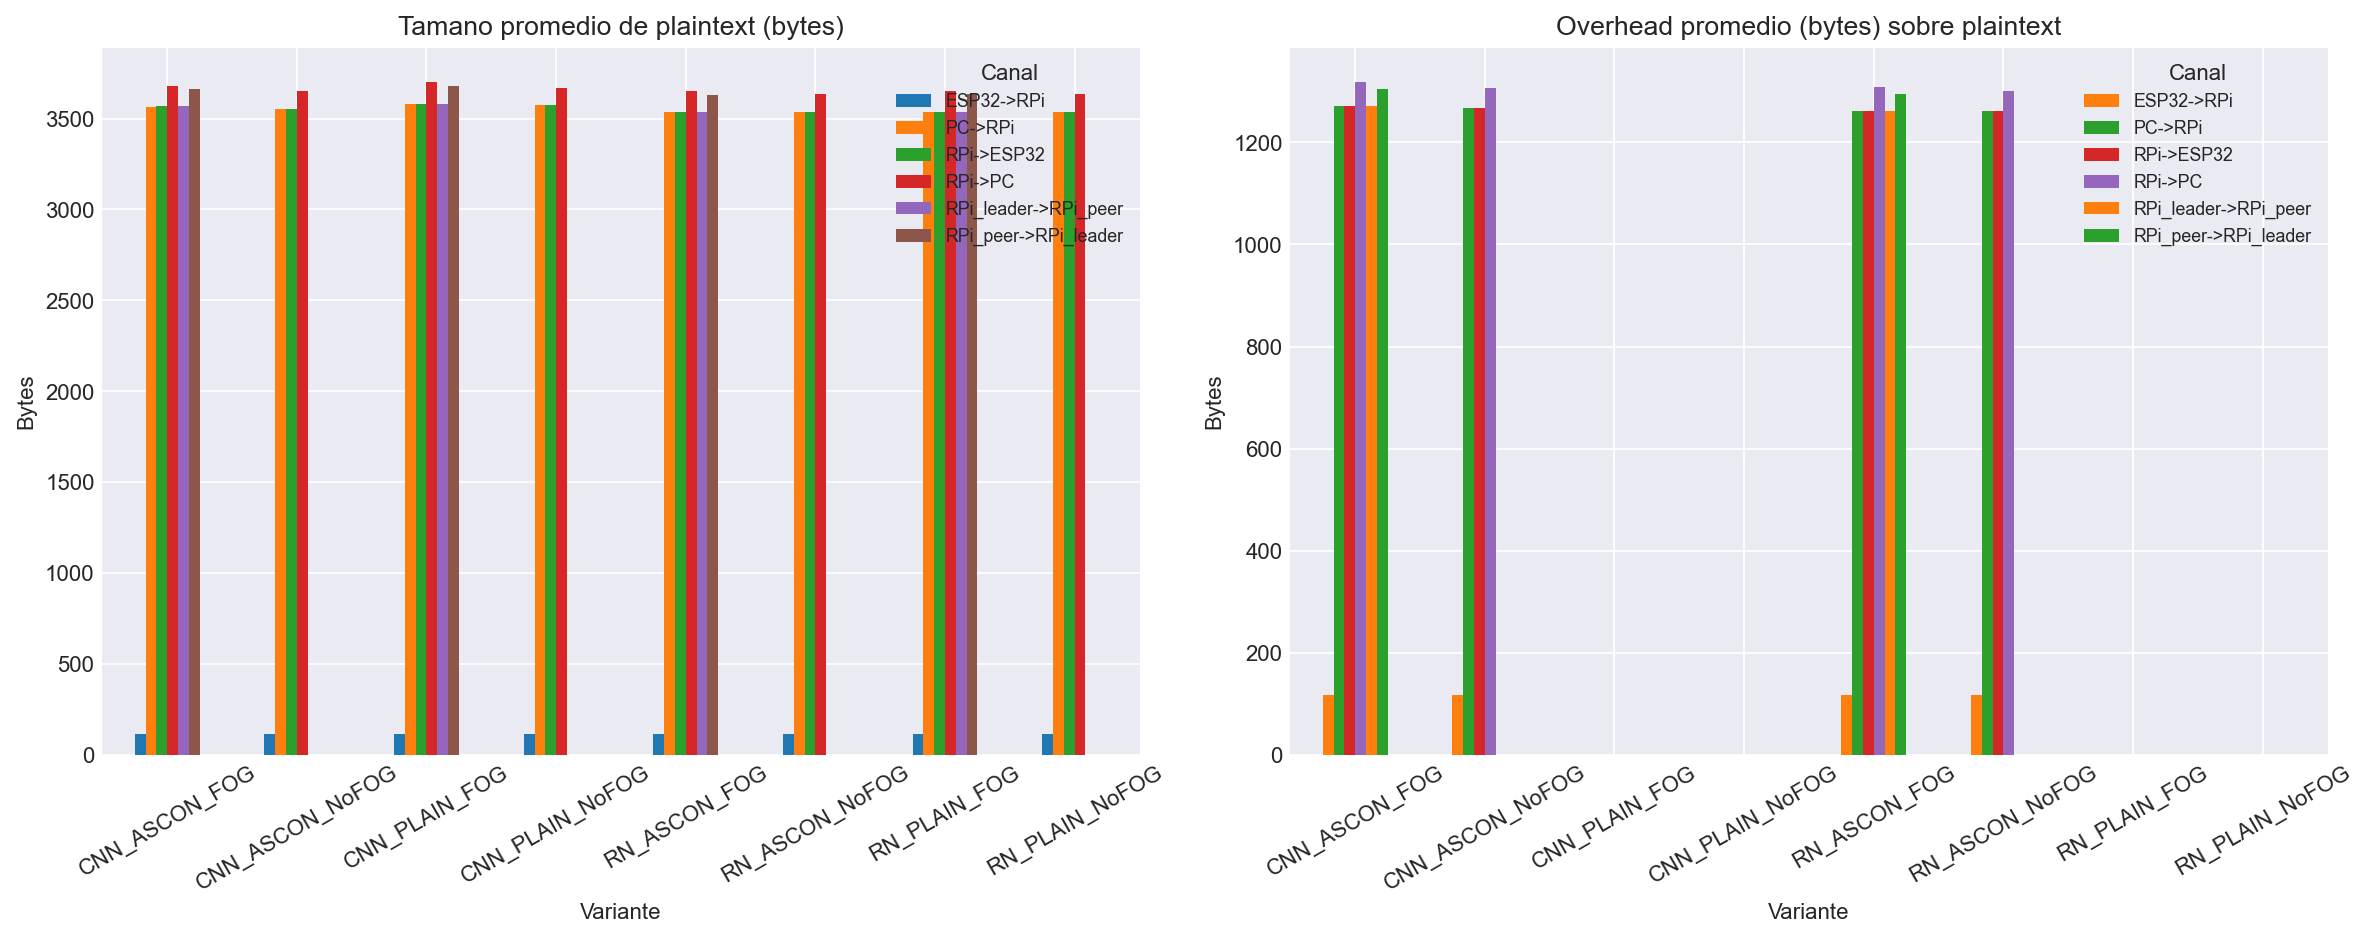
\includegraphics[width=\linewidth]{fig_payload.png}
    \caption{Mean payload size and ASCON envelope overhead per channel.}
  \end{subfigure}
  \caption{Per-channel cryptographic and communication overhead. PLAIN
  variants report only JSON serialisation time (sub-millisecond) and zero
  envelope overhead by construction.}
  \label{fig:overhead}
\end{figure}

ASCON-128 decryption at the ESP32-S3 gateway entry takes
4.4--4.7\,ms~p95, essentially independent of model and topology. At the
PC server the Python implementation reports 24--27\,ms~p95 in NoFOG and
37--50\,ms~p95 in FOG (the leader re-encrypts pre-aggregated updates,
which doubles the cryptographic operations on the upstream path). Summed
over a federated round, ASCON contributes between 73\,ms (NoFOG) and
140\,ms (FOG); over rounds of 51--73\,s this is between 0.10\,\% and
0.27\,\% of the round time (Fig.~\ref{fig:overhead}, left).

In terms of payload, the ASCON envelope adds on average 1.07\,kB per
message, or $\approx$48\,\% relative to a 2.25\,kB plaintext payload
(Table~\ref{tab:overhead_size}). This breaks down as a fixed 16-byte tag,
16-byte nonce, a $\times 4/3$ base64 expansion, and a $\sim$30-byte JSON
envelope. On a standard 54\,Mbps Wi-Fi link the absolute additional
transmission time per round (3.2\,kB in NoFOG, 5--6\,kB in FOG) is below
one millisecond and therefore negligible.

\begin{table}[t]
\centering
\caption{Size overhead per ASCON variant. PLAIN omitted (zero by
construction).}
\label{tab:overhead_size}
\small
\begin{tabular}{@{}lrrr@{}}
\toprule
Variant & Plaintext (B) & Overhead (B) & Ratio (\%) \\
\midrule
CNN ASCON FOG     & 2365 & 1098 & 46.5 \\
CNN ASCON NoFOG   & 2143 & 1049 & 48.9 \\
RN ASCON FOG      & 2323 & 1084 & 46.6 \\
RN ASCON NoFOG    & 2162 & 1050 & 48.5 \\
\midrule
\textbf{Mean}     & \textbf{2248} & \textbf{1070} & \textbf{47.6} \\
\bottomrule
\end{tabular}
\end{table}

\subsection{Federated vs.\ centralised}

Compared to the Random Forest centralised ceiling (0.9994), the best
federated variant reaches 0.9750, a 2.4-point gap. The MLP variants pay a
larger gap (5--6 points), consistent with the FL non-IID literature
\cite{imteaj2022survey,albanbay2025}. In exchange, the federated system
exchanges only 163~parameters (652~bytes) per round between each gateway
and the coordinator, compared with the millions of feature values that a
centralised collector would have to ingest --- a reduction in transferred
information of more than 99.99\,\%.

% =====================================================================
\section{Threats to Validity}
\label{sec:threats}

We make the following limitations explicit, because they constrain the
generalisability of the reported numbers.

\paragraph{Closed three-class label set.}
The system is a closed-set classifier over \emph{normal},
\emph{mqtt\_bruteforce} and \emph{scan\_A}. A traffic vector outside this
set (e.g.\ \emph{slowloris}, MQTT broker spoofing, application-layer DoS,
covert exfiltration over QoS-2) will be mapped to the closest known class
by softmax similarity, with two failure modes: a silent false negative if
it resembles \emph{normal}, or a noisy false positive if it resembles a
known attack class. Open-set recognition or an explicit anomaly-detection
head is required to mitigate this and is left as future work.

\paragraph{Heuristic gateway labelling.}
Labels at the gateway are assigned by fixed thresholds on
\texttt{num\_pkts}, \texttt{mean\_pkt\_len} and \texttt{num\_psh}
calibrated on the public datasets. This produces label noise relative to
the ground-truth annotations and partially accounts for the residual gap
versus the centralised baseline. A learned labelling head or a fully
ground-truthed real capture would tighten this bound.

\paragraph{Limited testbed scale.}
The reported numbers come from two gateways and four edge nodes,
sufficient to validate the cycle but not large enough to characterise
behaviour at the scale of dozens or hundreds of gateways. At larger scale
the PC coordinator would become a bottleneck and a genuinely distributed
Fog plane (multiple leaders or sharded topics) would be required.
Stronger non-IID distributions between gateways are also expected to
widen the gap to the centralised baseline.

\paragraph{Simulated traffic, no energy reporting.}
The ESP32-S3 nodes emit calibrated traffic rather than capturing real
MQTT flows. Energy consumption was not measured in the present setup;
both points are flagged in the future-work section.

\paragraph{Cryptographic threat model and key management.}
ASCON-128 is evaluated as a black-box AEAD. We did not perform side-channel
attacks (power analysis, EM, fault injection) against the implementation,
and the system assumes deployment in a physically controlled environment.
A 128-bit symmetric key is pre-shared across all devices to simplify the
prototype; a production deployment would require key rotation, secure
onboarding of new nodes and revocation of compromised devices, none of
which are addressed here. Mirzaali \textit{et~al.}~\cite{mirzaali2025lwc}
provide a methodological template for an active attack campaign on
Raspberry Pi that we intend to replicate as future work.

\paragraph{Statistical significance.}
Per-variant means are computed over 5--8 attempts. Variance and confidence
intervals are reported in the underlying telemetry CSVs but not in the
summary table for space reasons; absolute differences below approximately
1.5~percentage points should not be over-interpreted.

% =====================================================================
\section{Conclusions and Future Work}
\label{sec:conclusion}

We presented an Edge--Fog--Cloud intrusion-detection system for IoT/MQTT
networks that jointly evaluates TinyML inference on ESP32-S3,
hierarchical federated learning across Raspberry Pi~4 gateways, and
ASCON-128 authenticated encryption over the full federated cycle. Eight
configurations crossing model, security and topology were measured under
a unified telemetry layer over 58 federated runs. The best variant,
\texttt{CNN\_ASCON\_FOG}, reaches 0.975 global accuracy with an
ASCON-induced temporal overhead below 0.3\,\% of the round time and an
envelope size overhead of $\approx$48\,\% per message; the on-device
model footprint of $\approx$4.5\,kB leaves more than 60\,\% of the
ESP32-S3 SRAM free during operation. The Fog topology improves accuracy
when combined with ASCON but can degrade it without authentication,
suggesting that pre-aggregation is best deployed in conjunction with
end-to-end integrity guarantees.

The contribution should be read as a functional end-to-end proof of the
integration, not as a production-ready solution: the testbed is small, the
label set is closed, and the cryptographic deployment relies on a
pre-shared key. Three directions stand out as immediate future work. The
first is Byzantine-robust aggregation and stronger non-IID handling ---
FedProx, SCAFFOLD or hierarchical schemes such as EdgeTrust-Shard
\cite{li2020fedprox,tran2026edgetrust} --- to address the gap that real
deployments are likely to exhibit. The second is moving from the
pre-shared key used in this prototype to a realistic key-management plane
with rotation, secure onboarding and revocation, complemented by a
side-channel hardening campaign of the ASCON implementation along the
lines surveyed by Kaur~\textit{et~al.}~\cite{kaur2025ascon} and an active
attack replication in the spirit of Mirzaali
\textit{et~al.}~\cite{mirzaali2025lwc}. The third is widening the label
set beyond the three classes evaluated here (e.g.\ MQTT flooding, botnet
traffic, credential abuse) and pairing the closed-set classifier with an
open-set or anomaly detection head, so that traffic outside the trained
catalogue is flagged as unknown rather than mapped to the nearest known
class.

% =====================================================================
\bibliographystyle{splncs04}
\bibliography{paper}

\end{document}
